\section{Software architecture}\label{sec:softwareArchitecture}
In this section, the software architecture of MeltyFi is shown in detail. All the tools used are mentioned, an overview of all the protocol components is given, and then they are explained individually. Finally, reflections are given regarding the design choices made. 
\\
\indent The entire protocol is open-source and is searchable on GitHub \cite{MeltyFi}. It is also possible to interact with MeltyFiNFT via \href{https://goerli.etherscan.io/address/0x6c1030B8BbE523671Bcfd774Ae59ef620f9f31b4}{Goerli Etherscan interface} or \href{https://meltyfi.nft}{MeltyFi.NFT DApp}. Equally it is possible to interact with MeltyFiDAO via \href{https://goerli.etherscan.io/address/0xC4AA65a48fd317070F1A5aC5eBAC70F9d022Fb1e}{Goerli Etherscan interface} or \href{https://meltyfi.dao}{MeltyFi.DAO DApp}. MeltyFiNFT encapsulates the core of the MeltyFi protocol while MeltyFiDAO encapsulates the DAO management of the MeltyFi protocol.

\subsection{Tools used}
For the realization of the MeltyFi protocol we relied on the environment \textbf{Node.js} \cite{nodejs} in order to use the following npm packages:
\begin{itemize}
    \item \textbf{@openzeppelin/contracts}: used for draw on all the already audited code that we would use when necessary \cite{openzeppelin}
    \item \textbf{@chainlink/contracts}: used for the realization of the whole part that makes use of oracles \cite{chainlink}
    \item \textbf{hardhat}: used as development environment \cite{hardhat}
    \item \textbf{@nomicfoundation/hardhat-toolbox}: used to deploy on goerli testnet and verify contract on etherscan \cite{hardhattoolbox}
    \item \textbf{hardhat-docgen}: used for automatic generation of code documentation \cite{hardhatdocgen}
    \item \textbf{dotenv}: used to load sensible datas in the code such as private keys and API keys \cite{dotenv}
\end{itemize}
The \textbf{Alchemy API} \cite{alchemyapi} was used to make deployment possible, and the \textbf{Etherscan API} \cite{etherscanapi} was used to make contract verification possible. \textbf{Remix} \cite{remix} was used as an editor while writing the contracts. The latter were compiled with \textbf{solidity compiler 0.8.17}. Overall, all the MeltyFi protocol is capable of running on the same or higher versions of \textbf{solidity 0.8.9}. This choice made avoids overflow problems and allows us to benefit from all the audit code that was intended to be used. 
\\
\indent Finally, to allow MeltyFi to function properly, which requires interaction with oracles, the entire protocol was deployed on \textbf{Goerli testnet} \cite{goerlitestnet}. \textbf{Goerli faucet} \cite{goerlifaucet} and \textbf{Link faucet} \cite{linkfaucet} were used to enable this.

\subsection{Protocol blueprint}
The blueprint of the entire protocol is shown in \autoref{fig:Protocol_blueprint}. As already mentioned, \textbf{MeltyFiNFT} is the contract that handles all the main lending and borrowing part of the protocol. MeltyFiNFT is also a contract that handles an ERC-1155 token, this token is none other than WonkaBar (the utility token). MeltyFiNFT is owner of \textbf{LogoCollection} (the meme token) to be able to mint at the user's request, it is owner of \textbf{ChocoChip} (the governance token) to be able to mint when due, and finally it is owner of \textbf{VRFv2DirectFundingConsumer} to make a request for a random word to be able to elect the winner of a completed lottery. \textbf{MeltyFiDAO} is the contract that manages the DAO of the protocol, so it needs a \textbf{TimelockController} and CochoChip as the governance token.
\begin{figure}[h]
    \centering
    \includegraphics[width=0.6\textwidth]{figures/Protocol_blueprint.png}
    \caption{Protocol blueprint}
    \label{fig:Protocol_blueprint}
\end{figure}

\subsection{LogoCollection}
\begin{figure}[h]
    \centering
    \includegraphics[width=\textwidth]{figures/LogoCollection_class_diagram.png}
    \caption{LogoCollection.sol class diagram}
    \label{fig:LogoCollection}
\end{figure}
LogoCollection is an \textbf{ERC-1155} token whose supply can be monitored, minable only by the owner and burnable by anyone. This token has no utility, in fact it is intended to be the \textbf{meme token}, created to publicize the protocol logo. So that is why it is minable by anyone via the \texttt{mintLogo} function found in MeltyFiNFT. The ERC-1155 standard was used to take advantage of the fungibility of ERC-20 tokens and the ability to integrate metadata as is done in ERC-721 tokens. The \autoref{fig:LogoCollection} shows the class diagram of the LogoCollection contract, while the \autoref{fig:LogoCollectionImg} shows the image attached to the token. 
\begin{figure}[h]
    \centering
    \includegraphics[width=0.5\textwidth]{figures/LogoCollectionImg.jpg}
    \caption{LogoCollection}
    \label{fig:LogoCollectionImg}
\end{figure}

\subsection{ChocoChip}
\begin{figure}[h]
    \centering
    \includegraphics[width=\textwidth]{figures/ChocoChip_class_diagram.png}
    \caption{ChocoChip.sol class diagram}
    \label{fig:ChocoChip}
\end{figure}
The \autoref{fig:ChocoChip} shows the class diagram of the ChocoChip contract. ChocoChip (\$CHOC) is an \textbf{ERC-20} token whose supply can be monitored, minable only by the owner, and burnable by anyone. ChocoChip has the property of allowing approvals to occur through signatures. Being a \textbf{governance token}, ChocoChip must necessarily also have the snapshot and voting property. ChocoChip starts with a supply of zero units and can only be minted if capital is employed in the protocol. 
\\
\indent This is possible by buying WonkaBars or by repaying a loan. In the first case, buying WonkaBars is equivalent to buying tickets of active lotteries. In fact, when a lottery is concluded or cancelled, it will be possible to call the \texttt{meltWonakBars} function of MeltyFiNFT to melt your WonkaBars related to the concluded or cancelled lottery. Doing so will result in receiving 1 \$CHOC for each Finney spent in the purchase of the WonkaBars being melted. In fact, this is equivalent to receiving a prize equal to the capital spent in the protocol. 
\\
\indent In the second case, it is possible to receive ChocoChips if you repay a loan taken out with MeltyFiNFT. In fact, the borrower who creates a lottery, and then takes out a loan, will receive all earnings from the WonkaBars sold from that lottery, excluding a 5\% royalty that is earmarked for MeltyFiDAO's treasury. To repay the loan, the borrower will have to pay back an amount equal to the value of all WonkaBars sold (doing the math, the interest is 5.26\%). The difference between the full amount he pays back and the money he was actually loaned equals the value the borrower spent on the protocol and thus he will receive 1 \$CHOC for every Finney spent on the protocol. So the borrower receives a prize equal to the capital spent in the protocol. 
\\
\indent ChocoChip holders should be interested in holding the token because possession of the token itself demonstrates a kind of proof of work in having employed their capital in the protocol. However, a new ChocoChip is minted with each Finney employed in the protocol, and this feature allows the token to be backed in some sense to the value of \$ETH. In addition, ChocoChip is the governance token of MeltyFiDAO, the protocol's decentralized autonomous organization. This means that \$CHOC holders have decision-making power over protocol changes and updates based on the amount of \$CHOC they hold. Obviously, since \$CHOC is a token that demonstrates the holder's use of the protocol, it is correct to weigh votes based on the balance of \$CHOC to intrapreneur decisions about protocol changes. ChocoChip, besides being the perfect token to employ in the DAO of the protocol, is also the perfect token to distribute the value of the treasury among all ChocoChip holders. In fact, for every circulating ChocoChip, there is one Finney in MeltyFiDAO's treasury. After these considerations, it's possible to see that DAO could decide to make the treasury worthwhile and distribute the revenue to the ChocoChip holders. In short, those who hold \$CHOC will benefit proportionately from the proper use of the treasury and can make decisions about how to properly employ the treasury or how best to modify the protocol in a healthy way.

\subsection{TimelockController}
The \autoref{fig:TimelockController} shows the class diagram of the TimelockController contract. This contract is useful for the proper construction of MeltyFiDAO. Indeed, in a governance system, the TimelockController contract is responsible for introducing a delay between a proposal and its execution. 
\begin{figure}[h]
    \centering
    \includegraphics[width=0.3\textwidth]{figures/TimelockController_class_diagram.png}
    \caption{TimelockController.sol class diagram}
    \label{fig:TimelockController}
\end{figure}

\subsection{MeltyFiDAO}
\begin{figure}[h]
    \centering
    \includegraphics[width=\textwidth]{figures/MeltyFiDAO_class_diagram.png}
    \caption{MeltyFiDAO.sol class diagram}
    \label{fig:MeltyFiDAO}
\end{figure}
The \autoref{fig:MeltyFiDAO} shows the class diagram of the MeltyFiDAO contract. MeltyFiDAO was programmed following Openzeppelin's best practices, taking advantage of Openzeppelin's audit code for the most part precisely. MeltyFiDAO uses ChocoChip as the governance token, is Bravo compatible and has a TimelockController.

\subsection{VRFv2DirectFundingConsumer}
VRFv2DirectFundingConsumer is a fair and \textbf{verifiable random number generator}, provided by chainlink, that allows MeltyFiNFT to access random values without jeopardizing security. VRFv2DirectFundingConsumer is called to generate a random word to elect the winner of a lottery when it concludes. For each request MeltyFiNFT makes to VRFv2DirectFundingConsumerFor some \$LINK is spent from MeltyFiNFT's account. This is not a problem, it is the cost of the service. The \autoref{fig:VRFv2Consumer} shows the class diagram of the VRFv2DirectFundingConsumer contract.
\begin{figure}[h]
    \centering
    \includegraphics[width=0.6\textwidth]{figures/VRFv2DirectFundingConsumer_class_diagram.png}
    \caption{VRFv2DirectFundingConsumer.sol class diagram}
    \label{fig:VRFv2Consumer}
\end{figure}

\subsection{MeltyFiNFT}
\begin{figure}
    \centering
    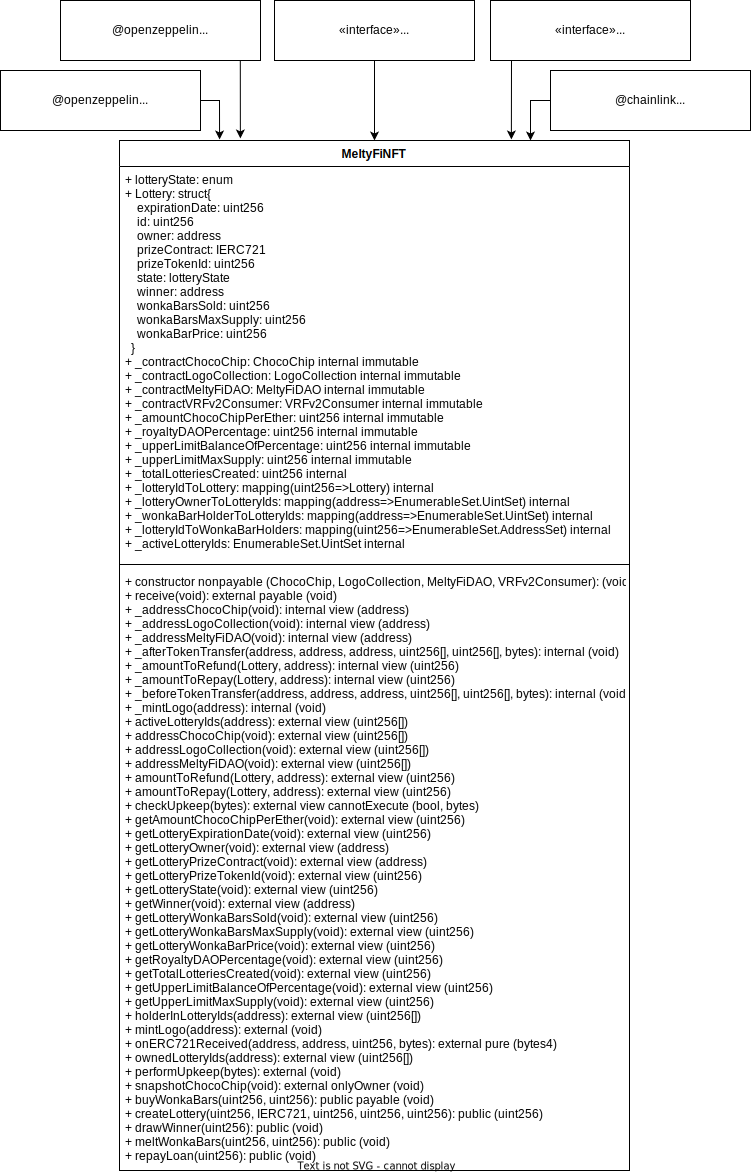
\includegraphics[width=\textwidth]{figures/MeltyFiNFT_class_diagram.png}
    \caption{MeltyFiNFT.sol class diagram}
    \label{fig:MeltyFiNFT}
\end{figure}
MeltyFiNFT is the contract that runs the core functionality of the MeltyFi protocol. It manages the creation, cancellation and conclusion of lotteries, as well as the sale and refund of WonkaBars for each lottery, and also reward good users with ChocoChips. The contract allows users to create a lottery by choosing their NFT to put as lottery prize, setting an expiration date and defining a price in Ether for each WonkaBar sold. When a lottery is created, the contract will be able to mint a fixed amount of WonkaBars (setted by lottery owner) for the lottery. These WonkaBars are sold to users interested in participating in the lottery and money raised are sent to the lottery owner (less some fees). Once the expiration date is reached, the contract selects a random WonkaBar holder as the winner, who receives the prize NFT. Plus every WonkaBar holder is rewarded with ChocoCips. If the lottery is cancelled by the owner beafore the expiration date, the contract refunds WonkaBars holders with Ether of the lottery owners. Plus every WonkaBar holder is rewarded with ChocoCips.
\\
\indent The \autoref{fig:MeltyFiNFT} shows the class diagram of the MeltyFiNFT contract. MeltyFiNFT extends the IERC721Receiver interface to allow the reception of ERC721 tokens. MeltyFi also extends the AutomationCompatibleInterface interface and the AutomationBase contract to enable the cunstom logic automation offered by chainlink, which is useful for ending a lottery when the expiration date is reached and then electing the NFT winner, i.e., the prize of the concluded lottery. MeltyFi also extends Ownable and ERC1155Supply for managing the WonkaBar token.

\subsubsection{WonkaBar}
WonkaBar (\$WKB) is a token \textbf{ERC-1155} managed by MeltyFiNFT to generate \textbf{lottery tickets} for each lottery. The ERC-1155 standard is perfect for generating lottery tickets, in fact to each WonkaBar token ID we match a lottery with the same token ID so that for each lottery we get specific WonkaBars. In fact for each token ID, WonkaBar stores the balance of all users who own the respective WonkaBars to that token ID, thus to the lottery with the same token ID as the WonkaBars. The \autoref{fig:WonkaBarImg} shows the image attached to the token. 
\begin{figure}[h]
    \centering
    \includegraphics[width=0.5\textwidth]{figures/WonkaBarImg.png}
    \caption{WonkaBar}
    \label{fig:WonkaBarImg}
\end{figure}
\subsubsection{Lottery}
Lottery is a structure maintained by MeltyFiNFT to hold all the useful information for each lottery. The structure is shown in detail below. Note that the lottery can have \textbf{four possible states}, described in detail in \autoref{fig:lotteryState} and commented on below. 
\\
\indent A lottery is \textbf{active} when it has been created, the lottery owner has not yet cancelled it (i.e., has not yet executed \texttt{repayLoan} on the lottery), and the expiration date has not yet passed. When a lottery is active, it is possible to buy WonkaBars of the said lottery. 
\\
\indent A lottery from active can become \textbf{cancelled} when the owner executes \texttt{repayLoan} before the expiration date and someone has bought WonkaBars from the lottery. If no one has bought lottery WonkaBars, then after \texttt{rapayLoan} the lottery is trashed. Of a cancelled lottery, holders of WonkaBars from that lottery can call \texttt{meltWonkaBars} to get back the money used in the purchase of WonkaBars and to get ChocoChips.
\\
\indent A lottery from active can become \textbf{concluded} if at the expiration date the owner has not yet repaid the loan and someone has bought WonkaBars from the lottery. If no one has bought lottery WonkaBars, then at the expiration date the lottery is trashed. Of a concluded lottery, holders of WonkaBars from that lottery can call \texttt{meltWonkaBars} to get ChocoChips. If \texttt{meltWonkaBars} is executed by the winner of the lottery, in addition to the ChocoChips, that winner also receives the NFT put in for the lottery.
\\
\indent A lottery is \textbf{trashed} when it has finished being active and there are no more (or never were) WonkaBar holders for that lottery.

\begin{figure}[h]
    \centering
    \includegraphics[width=0.6\textwidth]{figures/Lottery_state_diagram.png}
    \caption{Lottery state diagram}
    \label{fig:lotteryState}
\end{figure}
\begin{minted}[linenos,breaklines]{solidity}
/// Data type representing the possible states of a lottery
enum lotteryState {
    ACTIVE,
    CANCELLED,
    CONCLUDED,
    TRASHED
}
/// Struct for storing the information of a lottery
struct Lottery {
    /// Expiration date of the lottery, in seconds
    uint256 expirationDate;
    /// ID of the lottery
    uint256 id;
    /// Owner of the lottery
    address owner;
    /// Prize NFT contract of the lottery
    IERC721 prizeContract;
    /// Prize NFT token ID of the lottery
    uint256 prizeTokenId;
    /// State of the lottery
    lotteryState state;
    /// Winner of the lottery
    address winner;
    /// Number of WonkaBars sold for the lottery
    uint256 wonkaBarsSold;
    /// Maximum supply of WonkaBars for the lottery
    uint256 wonkaBarsMaxSupply;
    /// Price of each WonkaBar for the lottery, in wei
    uint256 wonkaBarPrice;
}
\end{minted}

\subsubsection{Data structures}
The following are descriptions of the data structures used by MeltyFi for proper operation. \texttt{\_lotteryIdToLottery} is used whenever you want to retrieve the data of a lottery starting from the lottery ID. \texttt{\_lotteryIdToWonkaBarHolders} is used in \texttt{drawWinner} to retrieve all the WonkaBar holders of the lottery whose winner you want to draw. \texttt{\_activeLotteryIds} is useful in \texttt{checkUpkeep} to figure out which active lotteries reach expire date, so as to perform the conclusion of these and elect the winner. \texttt{\_lotteryOwnerToLotteryIds} and \texttt{\_wonkaBarHolderToLotteryIds} are useful for retrieving hard-to-find data immediately, useful only for those using MeltyFiNFT or interfaces that implement MeltyFiNFT.
\begin{minted}[linenos,breaklines]{solidity}
/// maps a unique lottery ID to a "Lottery" object containing information about the lottery itself
mapping(uint256 => Lottery) internal _lotteryIdToLottery;
/// maps the address of a lottery owner to a set of lottery IDs that they own
mapping(address => EnumerableSet.UintSet) internal _lotteryOwnerToLotteryIds;
/// maps the address of a WonkaBar holder to a set of lottery IDs for which they have purchased a ticket
mapping(address => EnumerableSet.UintSet) internal _wonkaBarHolderToLotteryIds;
/// maps a lottery ID to a set of WonkaBar holder addresses that have purchased a ticket for that lottery
mapping(uint256 => EnumerableSet.AddressSet) internal _lotteryIdToWonkaBarHolders;
/// set that stores the IDs of all active lotteries
EnumerableSet.UintSet internal _activeLotteryIds;
\end{minted}

\subsubsection{createLottery function}
This public function creates a new lottery. The function raises error in the following cases:
\begin{itemize}
    \item Error if the caller is not the owner of the prize.
    \item Error if the maximum number of WonkaBars for sale is greater that the upper bound.
\end{itemize}
The function parameters are the following:
\begin{itemize}
    \item \textbf{duration}: The duration of the lottery, in seconds.
    \item \textbf{prizeContract}: The contract that holds the prize for this lottery.
    \item \textbf{prizeTokenId}: The token ID of the prize for this lottery.
    \item \textbf{wonkaBarPrice}: The price of a WonkaBar in this lottery.
    \item \textbf{wonkaBarsMaxSupply}: The maximum number of WonkaBars that can be sold in this lottery.
\end{itemize}
The function return the ID of the new lottery.
\begin{minted}[linenos,breaklines]{solidity}
function createLottery(
    uint256 duration,
    IERC721 prizeContract,
    uint256 prizeTokenId,
    uint256 wonkaBarPrice,
    uint256 wonkaBarsMaxSupply
) public returns (uint256) 
{
    /// The maximum number of WonkaBars for sale must not be greater than the upper bound
    /// The maximum number of WonkaBars for sale must not be lower than the lower bound
    /// transfer the prize to this contract
    /// create a new lottery
    /// update internal state
    /// return the ID of the new lottery
}
\end{minted}

\subsubsection{buyWonkaBars function}
This function allows a user to buy a specified amount of WonkaBars for a lottery. The caller must send the correct amount of Ether along with the transaction. A percentage of the total spending will be transferred to the MeltyFiDAO contract and the rest will be transferred to the owner of the lottery. The caller's balance of WonkaBars for the specified lottery will also be updated. The function raises errors in the following cases:
\begin{itemize}
    \item Error if the lottery is not really active.
    \item Error if after this purchease the total supply of WonkaBars will exceed the maximum supply allowed.
    \item Error if the caller's balance of WonkaBars for this lottery, after the purchase, will exceed the \texttt{\_upperLimitBalanceOfPercentage}.
    \item Error if the value sent is not enough to cover the cost of the WonkaBars.
\end{itemize}
The function parameters are the following:
\begin{itemize}
    \item \textbf{lotteryId}: The ID of the lottery for which the WonkaBars are being purchased.
    \item \textbf{amount}: The number of WonkaBars to be purchased.
\end{itemize}
\begin{minted}[linenos,breaklines]{solidity}
function buyWonkaBars(
    uint256 lotteryId, 
    uint256 amount
) public payable
{
    /// retrieve the lottery with the given ID
    /// calculate the total spending for the WonkaBars
    /// The lottery must be really active
    /// After this purchease the total supply of WonkaBars must not exceed the maximum supply allowed
    /// The caller's balance of WonkaBars for this lottery, after the purchase, must not exceed the _upperLimitBalanceOfPercentage
    /// The caller must sent anough amount of Ether to cover the cost of the WonkaBars
    /// transfer _royaltyDAOPercentage of the total spending to the MeltyFiDAO contract
    /// transfer the rest of the total spending to the owner of the lottery
    /// mint the WonkaBars for the caller
    /// update the total number of WonkaBars sold for the lottery
}
\end{minted}
\subsubsection{repayLoan function}
This function repays the loan for the given lottery ID. The caller of the function must be the owner of the lottery. The function raises errors in the following cases:
\begin{itemize}
    \item Error if the caller is not the owner of the lottery.
    \item Error if the value sent is not enough to repay the loan.
    \item Error if the lottery is not more active.
\end{itemize}
The function parameters are the following:
\begin{itemize}
    \item \textbf{lotteryId}: The id of the lottery to repay the loan for.
\end{itemize}
\begin{minted}[linenos,breaklines]{solidity}
function repayLoan(
    uint256 lotteryId
) public payable 
{
    /// retrieve the lottery with the given ID
    /// Calculate the total amount to be repaid
    /// The caller must be the owner of the lottery
    /// The caller must sent anough amount of Ether to repay the loan
    /// The lottery must be active
    /// Mint Choco Chips to the owner of the lottery
    /// Transfer the prize to the owner of the lottery
    /// Remove the lottery from the active lotteries
    /// set the expiration date to the current block timestamp
    /// If the total supply of WonkaBars is 0
        /// set the state to TRASHED
    /// else
        /// set the state to CANCELLED
}
\end{minted}
\subsubsection{drawWinner function}
This function draws the winner of a lottery. The function raises errors in the following cases:
\begin{itemize}
    \item Error if the lottery state is not active.
    \item Error if the lottery expiration date is not passed.
    \item Error if the VRF request for random words is not fulfilled.
\end{itemize}
The function parameters are the following:
\begin{itemize}
    \item \textbf{lotteryId}: The ID of the lottery.
\end{itemize}
\begin{minted}[linenos,breaklines]{solidity}
function drawWinner(
    uint256 lotteryId
) public 
{
    /// retrieve the lottery with the given ID
    /// The lottery state must be active
    // The lottery expiration date must be passed
    /// remove lottery from the active lotteries
    /// if there are no WonkaBar sold transfer prize to the owner, otherwise set lottery winner
        /// transfer prize to the owner if no tokens were sold
        /// set lottery state to trashed
    /// else
        /// The VRF request for random words must be fulfilled
        /// set lottery winner
        /// set lottery state to concluded
}
\end{minted}
\subsubsection{meltWonkaBars function}
This function allows a user to melt their WonkaBars of a specific lottery when this is no longer active. If the lottery is canceled the sender will receive the refund and ChocoChips. If the lottery is concluded the sender will receive ChocoChips, and the lottery prize if he is the winner. The function raises errors in the following cases:
\begin{itemize}
    \item Error if the user does not have enough WonkaBar balance to melt the given amount.
    \item Error if the lottery is trashed.
    \item Error if lottery is really active.
    \item Error if lottery is waiting to be concluded by the oracle.
\end{itemize}
The function parameters are the following:
\begin{itemize}
    \item \textbf{lotteryId}: The ID of the lottery from which the WonkaBars will be melted.
    \item \textbf{amount}: The amount of WonkaBars to be melted.
\end{itemize}
\begin{minted}[linenos,breaklines]{solidity}
function meltWonkaBars(
    uint256 lotteryId, 
    uint256 amount
) public 
{
    /// retrieve the lottery with the given ID
    /// calculate the total refound for the WonkaBars
    /// the user must have enough WonkaBar balance to melt the given amount
    /// the lottery must not be trashed
    /// lottery must not be really active or waiting to be concluded by the oracle
    /// Burn the WonkaBars for the caller
    /// Mint Choco Chips to the caller
    /// if lottery state is cancelled, also refound the caller
    /// if the caller is the winner and he does not already receive the price
        /// transfer prize to the caller (the winner)
    /// if all lottery's WonkaBars are melted, trash the lottery
}
\end{minted}


\subsection{Deepening of the design choices}

\paragraph{Delegate call issue}
Delegate call was not used to transfer the ownership of LogoCollection, ChocoChips, VRFv2DirectFoundingConsumer to MeltyFiNFT, but it was done manually. It would have been convenient to use delegate call at the time of the constuction of MeltyFiNFT so that the ownership of all three contracts could be transferred to meltyFiNFT, but it was not able. 

\paragraph{Merge dilemma between MeltyFiNFT and WonkaBar}
It was considered several times during the outlining of the code structure whether or not to merge the contract that handled MeltyFiNFT with the one that handled WonkaBar. In the end, the solution was that they necessarily needed to be merged because otherwise there would be data inconsistency when WonkaBars were sent to address zero or simply when they were passed from one wallet to another MeltyFiNFT would store the old owner and not update this information. It was necessary to make these two contracts talk tightly
 if they were separate, so the decision that was made was to merge the two contracts to easily have consistency of all the data that the protocol needs to work properly. So WonkaBar and MeltyFiNFT effected the merge. Note also that with the merge it is then possible to easily update the data managed by MeltyFiNFT related to the WonkaBars hand in hand with the data itself of the WonkaBar token, this just in the \texttt{\_beforeTokenTransfer} and \texttt{\_afterTokenTransfer} functions.

\paragraph{WonkaBar sold and WonkaBar supply are different things}
For each lottery it is necessary to know both the WonkaBar supply of the relevant lottery and the WonkaBars sold. These two data may not have the same value when, for example, some WonkaBars are sent to address zero. In this case the WonkaBars sold would appear greater than the supply, and if the supply was used to calculate the WonkaBars sold, after some WonkaBars were sent to address zero, it would result in the borrower paying less than he should. One therefore needs both pieces of data. WonkaBar sold is useful for calculating exactly how many WonkaBars were sold (thus how many were mint) while WonkaBar supply is useful for figuring out whether a lottery is to be trashared or not. WonkaBar sold and WonkaBar supply are two data therefore that we need, they play two different roles and can be altered differently.

\paragraph{Looking for the best data structures}
The EnumerateSet data structures provided by Openzeppelin were used to rely on as much audited code as possible when possible, also making programming easier without having to think about building basic data structures for storing information. so only more complex, non-standard structures were built. These structures are all MeltyFi maps and they are all necessary, each essential for at least one function. 
\\
\indent There had also been thought of creating mapping mappings etc. To partition well all lottery related info by doing lottery state discrimination. but this was not good as an approach because solidity is not possible to do swaps of mappings but only of type date base (it would have been very complex to effect a lottery state change). So we focused more and more on formulating simple mappings that are indispensable to the operation and use of the protocol without storing derivable data. 

\paragraph{Lottery constraints}
It is necessary to make use of \_upperLimitBalanceOfPercentage to avoid disinterest in buying WonkaBar in a lottery where only one address holds too much probability of winning and \_upperLimitMaxSupply to avoid too long loop in the drawWinner, also a minimum limit of WonkaBar is needed to allow at least a minimum of 1 ticket per user. Then a min of 5 ticket for 25\% of \_upperLimitBalanceOfPercentage.

\paragraph{MeltyFi is safe without oracles} 
MeltyFi does not rely on any external factors except the interaction with the Chainlink oracles. What happens if the oracles do not do their duty? Maybe because they are late or maybe because the \$LINKs are missing in the accounts that fund the oracles. What happens is that you do not compromise the protocol because the consistency of the data remains intact and you would only delay the execution of the draw winner of the concluded lotteries. As to who is to fund link the oracles, the cunstom logic automation \cite{oracleautomation} must necessarily rely on an address that actively sends funds to chainlink, so it must necessarily be the address of the protocol deployer. Note that even if the protocol deployer does not fund the oracle with the \$LINKs, it is still possible to call \texttt{drawWinner}, because precisely cunstom logic automation is not strictly necessary, since it is just an automation of a call of \texttt{drawWinner}, which however can be done by anyone when the time comes to be able to do it. For the generation of the random number (for the drawing of the lottery winner) the oracle is necessarily needed, and a direct funding \cite{oraclerandom} was specifically chosen so that if the deployer does not fund the oracles, anyone can fund it in order to be able to enable the execution of \texttt{drawWinner}. So the protocol even if the deployer lacks funding or if the oracles delay execution, the protocol is not compromised.

\paragraph{Deploy best practice}
Obviously to deploy all the protocol contracts we chose to deploy them singly following the order dictated by the inter-contractual dependencies. Of course, it was not chosen to deploy a single contract that would deploy others; it would have been too costly unnecessarily.

\paragraph{No snapshot for WonkaBar token at the lotteries conclusion}
A snapshot of the WonkaBars is not taken when the lotteries expire (conclude) because it is not essential anyway and the way the protocol is structured it is not necessary.